%%%%%%%%%%%%%%%%%%%%%%%%%%%%%%%%%%%%%%%%%
% Arsclassica Article
% LaTeX Template
% Version 1.1 (1/8/17)
%
% This template has been downloaded from:
% http://www.LaTeXTemplates.com
%
% Original author:
% Lorenzo Pantieri (http://www.lorenzopantieri.net) with extensive modifications by:
% Vel (vel@latextemplates.com)
%
% License:
% CC BY-NC-SA 3.0 (http://creativecommons.org/licenses/by-nc-sa/3.0/)
%
%%%%%%%%%%%%%%%%%%%%%%%%%%%%%%%%%%%%%%%%%

%----------------------------------------------------------------------------------------
%	PACKAGES AND OTHER DOCUMENT CONFIGURATIONS
%----------------------------------------------------------------------------------------

\documentclass[
11pt, % Main document font size
a4paper, % Paper type, use 'letterpaper' for US Letter paper
oneside, % One page layout (no page indentation)
%twoside, % Two page layout (page indentation for binding and different headers)
headinclude,footinclude, % Extra spacing for the header and footer
BCOR5mm, % Binding correction
]{scrartcl}

%%%%%%%%%%%%%%%%%%%%%%%%%%%%%%%%%%%%%%%%%
% Arsclassica Article
% Structure Specification File
%
% This file has been downloaded from:
% http://www.LaTeXTemplates.com
%
% Original author:
% Lorenzo Pantieri (http://www.lorenzopantieri.net) with extensive modifications by:
% Vel (vel@latextemplates.com)
%
% License:
% CC BY-NC-SA 3.0 (http://creativecommons.org/licenses/by-nc-sa/3.0/)
%
%%%%%%%%%%%%%%%%%%%%%%%%%%%%%%%%%%%%%%%%%

%----------------------------------------------------------------------------------------
%	REQUIRED PACKAGES
%----------------------------------------------------------------------------------------

\usepackage[
nochapters, % Turn off chapters since this is an article        
beramono, % Use the Bera Mono font for monospaced text (\texttt)
%eulermath,% Use the Euler font for mathematics
pdfspacing, % Makes use of pdftex’ letter spacing capabilities via the microtype package
dottedtoc % Dotted lines leading to the page numbers in the table of contents
]{classicthesis} % The layout is based on the Classic Thesis style

\usepackage{arsclassica} % Modifies the Classic Thesis package

\usepackage[T1]{fontenc} % Use 8-bit encoding that has 256 glyphs

\usepackage[utf8]{inputenc} % Required for including letters with accents

\usepackage{graphicx} % Required for including images
\graphicspath{{Figures/}} % Set the default folder for images

\usepackage{enumitem} % Required for manipulating the whitespace between and within lists

\usepackage{lipsum} % Used for inserting dummy 'Lorem ipsum' text into the template

% \usepackage{subfig} % Required for creating figures with multiple parts (subfigures)

\usepackage{amsmath,amssymb,amsthm} % For including math equations, theorems, symbols, etc

\usepackage{varioref} % More descriptive referencing




%----------------------------------------------------------------------------------------
% MY PACKAGES
%----------------------------------------------------------------------------------------
\usepackage{microtype}
%\usepackage{tgheros}
%%% uni formatting
%\renewcommand{\familydefault}{\sfdefault} % when reverting back add eulermath to classicthesis option
\usepackage{newtxsf}
\linespread{1.15}
\usepackage{lineno}


% code to stop section line numbering from substack
% Source - https://tex.stackexchange.com/a/635606
% Posted by Jinwen
% Retrieved 2026-09-03, License - CC BY-SA 4.0
\newif\ifLNturnsON
\def\LocallyStopLineNumbers{\LNturnsONfalse%
	\ifLineNumbers\LNturnsONtrue\fi\nolinenumbers}
\def\ResumeLineNumbers{\ifLNturnsON\linenumbers\fi}

\makeatletter

\titleformat{\section}
{\LocallyStopLineNumbers\normalfont\Large\bfseries}{\thesection}{1em}{}[\ResumeLineNumbers]
\titleformat{\subsection}
{\LocallyStopLineNumbers\normalfont\large\bfseries}{\thesubsection}{1em}{}[\ResumeLineNumbers]
\titleformat{\subsubsection}
{\LocallyStopLineNumbers\normalfont\normalsize\bfseries}{\thesubsubsection}{1em}{}[\ResumeLineNumbers]
\titleformat{\paragraph}[runin]
{\LocallyStopLineNumbers\normalfont\normalsize\bfseries}{\theparagraph}{1em}{}[\ResumeLineNumbers]
\titleformat{\subparagraph}[runin]
{\LocallyStopLineNumbers\normalfont\normalsize\bfseries}{\thesubparagraph}{1em}{}[\ResumeLineNumbers]
%%% end of uni formatting

\usepackage[mathlf]{MinionPro} % onlytext
\usepackage{float}
%\usepackage[margin=3cm]{geometry}   % for non-printing
\usepackage[twoside,inner=3.5cm,outer=2.5cm,top=3cm,bottom=3cm]{geometry}
\usepackage{subcaption}
\usepackage{caption}
\captionsetup{
	format=plain,      % don't use the hanging/justified style
	justification=justified,
	singlelinecheck=false,
	labelsep=colon,    % "Figure 1: " inline before the text
	labelfont=bf,      % optional — bold "Figure 1:"
	textfont=normalfont
}

\usepackage[style=authoryear,
 maxbibnames=10,
 minbibnames=10,
 maxcitenames=2]{biblatex}
 
 % italicised 'et al.' from stackexchange:
 \renewbibmacro*{name:andothers}{% Based on name:andothers from biblatex.def
 	\ifboolexpr{
 		test {\ifnumequal{\value{listcount}}{\value{liststop}}}
 		and
 		test \ifmorenames
 	}
 	{\ifnumgreater{\value{liststop}}{1}
 		{\finalandcomma}
 		{}%
 		\andothersdelim\bibstring[\emph]{andothers}}
 	{}}
 	
 	\setlength\bibitemsep{0.4\baselineskip} % spacing in reference list
 
\addbibresource{references.bib}
\usepackage{siunitx}
\usepackage{gensymb}
\usepackage{nicefrac}
\usepackage{tabularx}
\usepackage[table]{xcolor}
\usepackage{acro}
\usepackage{tikz}





%----------------------------------------------------------------------------------------
%	THEOREM STYLES
%---------------------------------------------------------------------------------------

\theoremstyle{definition} % Define theorem styles here based on the definition style (used for definitions and examples)
\newtheorem{definition}{Definition}

\theoremstyle{plain} % Define theorem styles here based on the plain style (used for theorems, lemmas, propositions)
\newtheorem{theorem}{Theorem}

\theoremstyle{remark} % Define theorem styles here based on the remark style (used for remarks and notes)

%----------------------------------------------------------------------------------------
%	HYPERLINKS
%---------------------------------------------------------------------------------------

\hypersetup{
%draft, % Uncomment to remove all links (useful for printing in black and white)
colorlinks=true, breaklinks=true, bookmarks=true,bookmarksnumbered,
urlcolor=webbrown, linkcolor=RoyalBlue, citecolor=webgreen, % Link colors
pdftitle={}, % PDF title
pdfauthor={\textcopyright}, % PDF Author
pdfsubject={}, % PDF Subject
pdfkeywords={}, % PDF Keywords
pdfcreator={pdfLaTeX}, % PDF Creator
pdfproducer={LaTeX with hyperref and ClassicThesis} % PDF producer
}



%----------------------------------------------------------------------------------------
%	ACRONYMS
%---------------------------------------------------------------------------------------




\DeclareAcronym{ET}{
	short=ET,
	long=Evapotranspiration,
}
\DeclareAcronym{SHAP}{
	short=SHAP,
	long=SHapley Additive exPlanations,
}
\DeclareAcronym{ML}{
	short=ML,
	long=Machine Learning,
}
\DeclareAcronym{RF}{
	short=RF,
	long=Random Forest,
}
\DeclareAcronym{DL}{
	short=DL,
	long=Deep Learning,
}
\DeclareAcronym{EC}{
	short=EC,
	long=Eddy Covariance,
}
\DeclareAcronym{PAM}{
	short=PAM,
	long=Partitioning Around Medoids,
}
\DeclareAcronym{R2}{
	short={$R^2$},
	long=Coefficient of determination,
}
\DeclareAcronym{RMSE}{
	short=RMSE,
	long=Root Mean Square Error,
}
\DeclareAcronym{MAE}{
	short=MAE,
	long=Mean Absolute Error,
}
\DeclareAcronym{LOGO}{
	short=LOGO,
	long=Leave One Group Out,
}
\DeclareAcronym{NEP}{
	short=NEP,
	long=Net Ecosystem Productivity,
}
\DeclareAcronym{LAI}{
	short=LAI,
	long=Leaf Area Index,
}
\DeclareAcronym{RNN}{
	short=RNN,
	long=Recurrent Neural Network,
}
\DeclareAcronym{ANN}{
	short=ANN,
	long=Artificial Neural Network,
}
\DeclareAcronym{SVM}{
	short=SVM,
	long=Support Vector Machine,
}
\DeclareAcronym{RS}{
	short=RS,
	long=Remote Sensing,
}
\DeclareAcronym{VPD}{
	short=VPD,
	long=Vapour Pressure Deficit,
}
\DeclareAcronym{SC}{
	short={$g_s$},
	long=Stomatal Conductance,
}


 % Include the structure.tex file which specified the document structure and layout

\hyphenation{Fortran hy-phen-ation} % Specify custom hyphenation points in words with dashes where you would like hyphenation to occur, or alternatively, don't put any dashes in a word to stop hyphenation altogether

%----------------------------------------------------------------------------------------
%	TITLE AND AUTHOR(S)
%----------------------------------------------------------------------------------------

\title{} % The article title

%\subtitle{Subtitle} % Uncomment to display a subtitle

\author{} % The article author(s) - author affiliations need to be specified in the AUTHOR AFFILIATIONS block

\date{} % An optional date to appear under the author(s)

%----------------------------------------------------------------------------------------

\begin{document}
	\begin{titlepage} % Suppresses displaying the page number on the title page and the subsequent page counts as page 1
	\vspace*{1em} % star for top of page
	\newcommand{\HRule}{\rule{\linewidth}{0.5mm}} 
	
	\centering	
	
\includegraphics[scale=3.5]{uni_logo.png}
	\vspace{3em}

	\rule[0.5ex]{\linewidth}{2pt}\vspace*{-\baselineskip}\vspace*{3.2pt}
	\rule[0.5ex]{\linewidth}{1pt}\\[\baselineskip]
	\spacedallcaps{\Large Impacts of Forest Age on Spatial and Temporal Generalisation of Random Forest Evapotranspiration models}

	\rule[0.5ex]{\linewidth}{1pt}\vspace*{-\baselineskip}\vspace{3.2pt}
	\rule[0.5ex]{\linewidth}{2pt}
	
	\vspace{1.5em}
	
	\begin{minipage}{0.4\textwidth}
		\begin{flushleft}
			\large
			\textit{Author}\\
			Archie \textsc{Benn} % Your name
		\end{flushleft}
	\end{minipage}
	~
	\begin{minipage}{0.4\textwidth}
		\begin{flushright}
			\large
			\textit{Supervisor}\\
			Professor Martin \textsc{De Kauwe} % Supervisor's name
		\end{flushright}
	\end{minipage}
	
	\vspace{3em}
	\begin{abstract} 
		{\noindent{\textsc{Abstract}}}
		\newline
		
	\end{abstract}
	
	\vfill
	
	A dissertation submitted to the University of Bristol in accordance with
	the requirements of the degree of Master of Science by advanced study
	in Bioinformatics in the Faculty of Health and Life Sciences.
	
	\let\thefootnote\relax\footnotetext{* \textit{Department of Biology, University of Examples, London, United Kingdom}}
	
	\let\thefootnote\relax\footnotetext{\textsuperscript{1} \textit{Department of Chemistry, University of Examples, London, United Kingdom}}
	
	\vspace{2em}
\end{titlepage}
%----------------------------------------------------------------------------------------
%	HEADERS
%----------------------------------------------------------------------------------------

\renewcommand{\sectionmark}[1]{\markright{\spacedlowsmallcaps{#1}}} % The header for all pages (oneside) or for even pages (twoside)
%\renewcommand{\subsectionmark}[1]{\markright{\thesubsection~#1}} % Uncomment when using the twoside option - this modifies the header on odd pages
\lehead{\mbox{\llap{\small\thepage\kern1em\color{halfgray} \vline}\color{halfgray}\hspace{0.5em}\rightmark\hfil}} % The header style

\pagestyle{scrheadings} % Enable the headers specified in this block

%----------------------------------------------------------------------------------------
%	TABLE OF CONTENTS & LISTS OF FIGURES AND TABLES
%----------------------------------------------------------------------------------------

\maketitle % Print the title/author/date block

\setcounter{tocdepth}{2} % Set the depth of the table of contents to show sections and subsections only

\tableofcontents % Print the table of contents

\listoffigures % Print the list of figures

\listoftables % Print the list of tables

%----------------------------------------------------------------------------------------
%	ABSTRACT
%----------------------------------------------------------------------------------------

\section*{Abstract} % This section will not appear in the table of contents due to the star (\section*)



%----------------------------------------------------------------------------------------
%	AUTHOR AFFILIATIONS
%----------------------------------------------------------------------------------------

%----------------------------------------------------------------------------------------

\newpage % Start the article content on the second page, remove this if you have a longer abstract that goes onto the second page

%----------------------------------------------------------------------------------------
%	INTRODUCTION
%----------------------------------------------------------------------------------------

\section{Introduction}

A statement requiring citation \cite{Figueredo:2009dg}.


Some mathematics in the text: $\cos\pi=-1$ and $\alpha$.
 
%----------------------------------------------------------------------------------------
%	METHODS
%----------------------------------------------------------------------------------------

\section{Methods}



\begin{enumerate}[noitemsep] % [noitemsep] removes whitespace between the items for a compact look
\item First item in a list
\item Second item in a list
\item Third item in a list
\end{enumerate}

%------------------------------------------------

\subsection{Paragraphs}



\paragraph{Paragraph Description} \lipsum[7] % Dummy text

\paragraph{Different Paragraph Description} \lipsum[8] % Dummy text

%------------------------------------------------

\subsection{Math}



\begin{equation}
\cos^3 \theta =\frac{1}{4}\cos\theta+\frac{3}{4}\cos 3\theta
\label{eq:refname2}
\end{equation}

\lipsum[5] % Dummy text

\begin{definition}[Gauss] 
To a mathematician it is obvious that
$\int_{-\infty}^{+\infty}
e^{-x^2}\,dx=\sqrt{\pi}$. 
\end{definition} 

\begin{theorem}[Pythagoras]
The square of the hypotenuse (the side opposite the right angle) is equal to the sum of the squares of the other two sides.
\end{theorem}

\begin{proof} 
We have that $\log(1)^2 = 2\log(1)$.
But we also have that $\log(-1)^2=\log(1)=0$.
Then $2\log(-1)=0$, from which the proof.
\end{proof}

%----------------------------------------------------------------------------------------
%	RESULTS AND DISCUSSION
%----------------------------------------------------------------------------------------

\section{Results and Discussion}

\begin{figure}[H]
	\frame{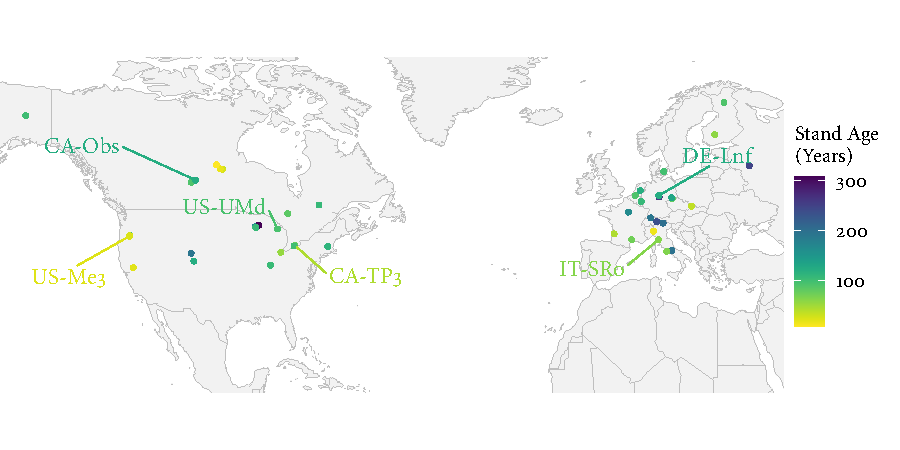
\includegraphics[width=\linewidth]{../figures/world_sites.pdf}}
	\captionsetup{justification=centering}
	\caption{Map of FLUXNET sites and associated stand age in this study}
\end{figure}



%------------------------------------------------

\subsection{Subsection}



\subsubsection{Subsubsection}



\begin{description}
\item[Word] Definition
\item[Concept] Explanation
\item[Idea] Text
\end{description}



\begin{itemize}[noitemsep] % [noitemsep] removes whitespace between the items for a compact look
\item First item in a list
\item Second item in a list
\item Third item in a list
\end{itemize}

\subsubsection{Table}



\begin{table}[hbt]
\caption{Table of Grades}
\centering
\begin{tabular}{llr}
\toprule
\multicolumn{2}{c}{Name} \\
\cmidrule(r){1-2}
First name & Last Name & Grade \\
\midrule
John & Doe & $7.5$ \\
Richard & Miles & $2$ \\
\bottomrule
\end{tabular}
\label{tab:label}
\end{table}

Reference to Table~\vref{tab:label}. % The \vref command specifies the location of the reference

%------------------------------------------------

\subsection{Figure Composed of Subfigures}

Reference the figure composed of multiple subfigures as Figure~\vref{fig:esempio}. Reference one of the subfigures as Figure~\vref{fig:ipsum}. % The \vref command specifies the location of the reference


%----------------------------------------------------------------------------------------
%	BIBLIOGRAPHY
%----------------------------------------------------------------------------------------

\renewcommand{\refname}{\spacedlowsmallcaps{References}} % For modifying the bibliography heading

\bibliographystyle{unsrt}

\bibliography{references.bib} % The file containing the bibliography

%----------------------------------------------------------------------------------------

\end{document}